\appendix
\section{Schaltpläne}
\label{sec:Schaltplan}
\subsection{Schaltplan Übersicht}
\begin{figure}[H]
	\centering
	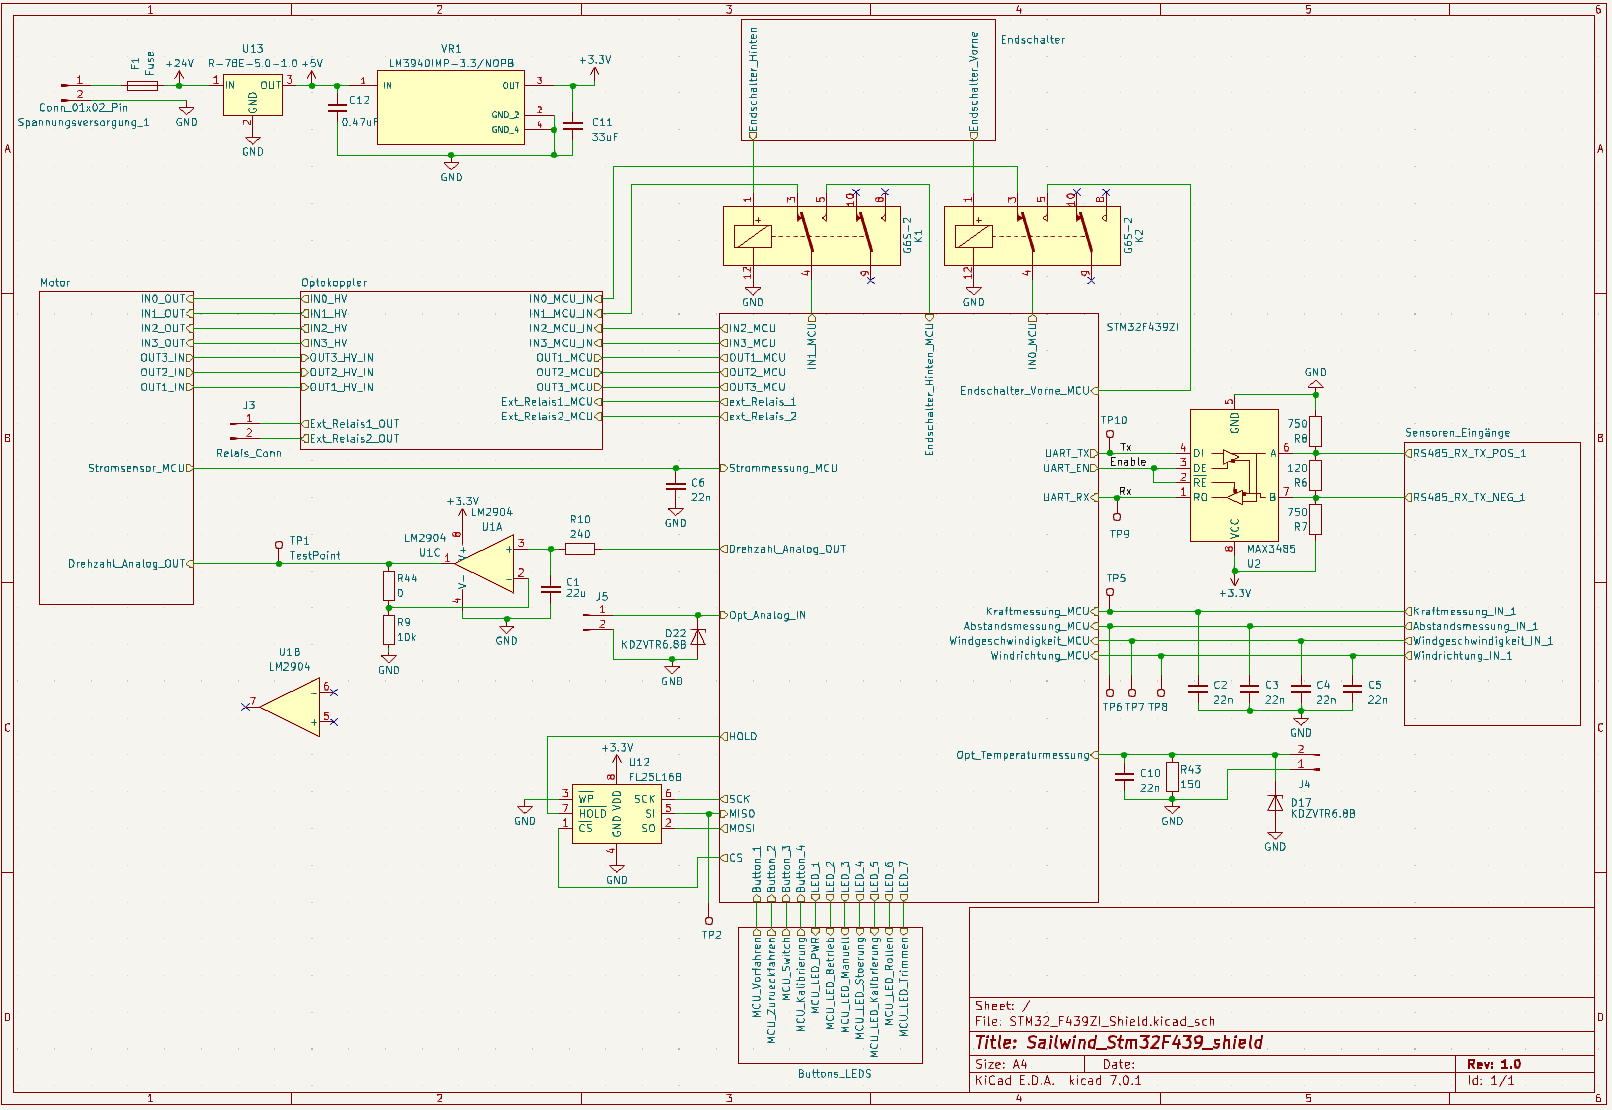
\includegraphics[width=1.0\textwidth]{images/Hardware/Schaltplan_Gesamt.PNG}
	\caption{Schaltplan Übersicht}
	\label{fig:Schaltplanuebersicht}\begin{center}
	\end{center}
\end{figure}
\subsection{Schaltplan STM32F439 Gruppe}
\begin{figure}[H]
	\centering
	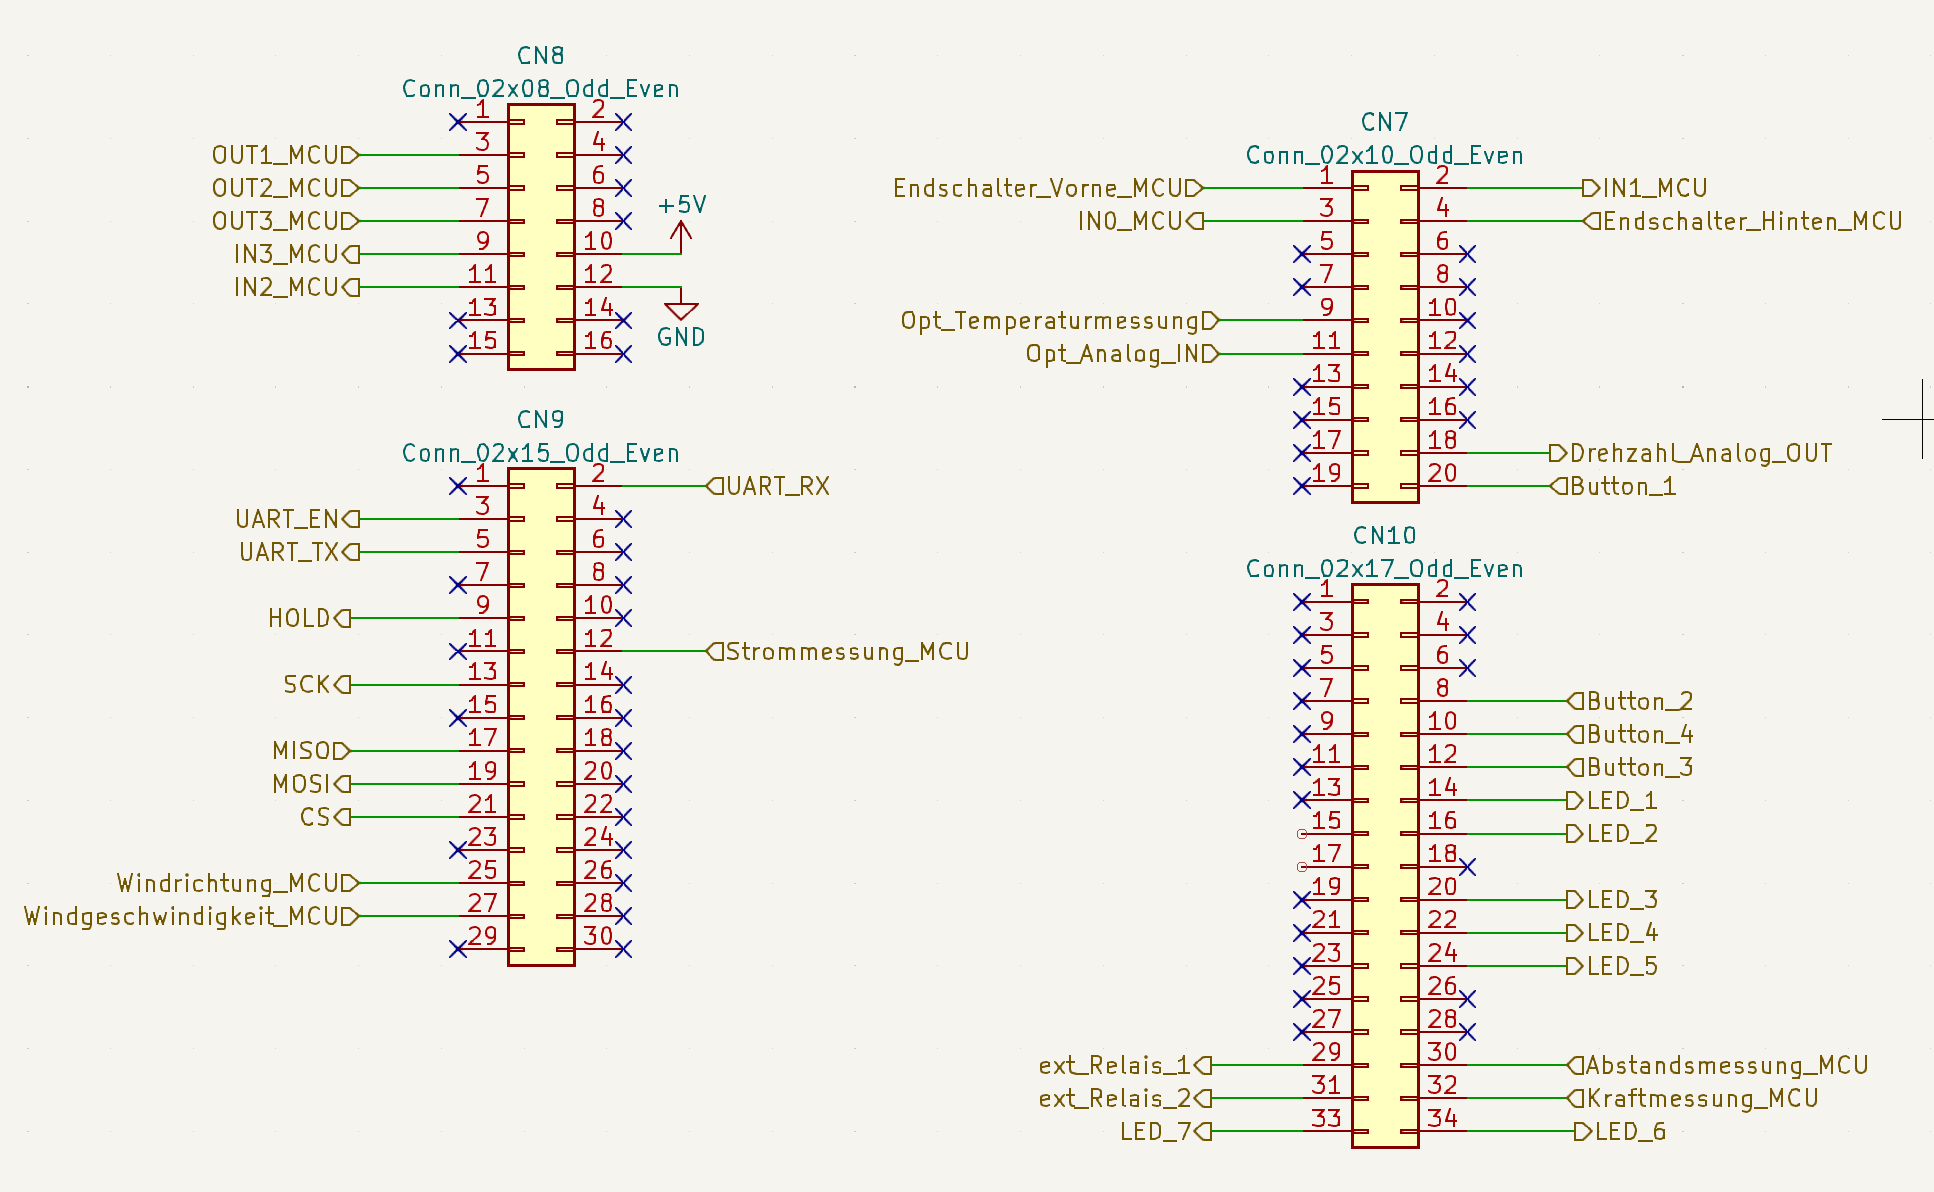
\includegraphics[width=1.0\textwidth]{images/Hardware/Schaltplan_STM32.PNG}
	\caption{Schaltplan der STM32F439 Gruppe}
	\label{fig:STM32Gruppe}\begin{center}´
	\end{center}
\end{figure}
\subsection{Schaltplan Buttons und LED Gruppe}
\begin{figure}[H]
	\centering
	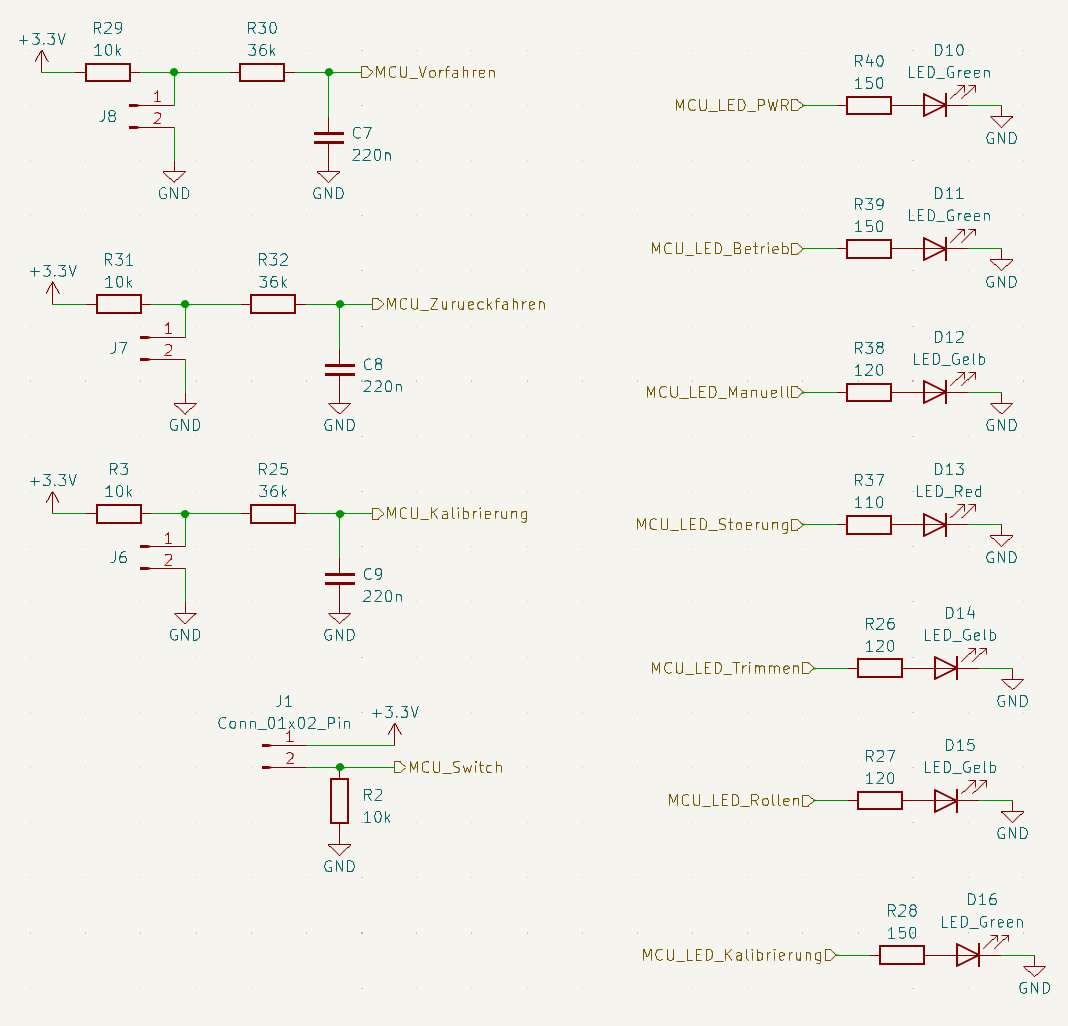
\includegraphics[width=1.0\textwidth]{images/Hardware/LEDS_und_buttons_schaltplan.PNG}
	\caption{Schaltplan der Buttons und LED Gruppe}
	\label{fig:ButtonGruppe}\begin{center}
	\end{center}
\end{figure}
\subsection{Schaltplan Sensoren Gruppe}
\begin{figure}[H]
	\centering
	\includegraphics[width=1.0\textwidth]{images/Hardware/Sensoren_Eingänge_Schaltplan.PNG}
	\caption{Schaltplan der Sensoren Gruppe}
	\label{fig:SensorenGruppe}\begin{center}
	\end{center}
\end{figure}
\subsection{Schaltplan Motor Gruppe}
\begin{figure}[H]
	\centering
	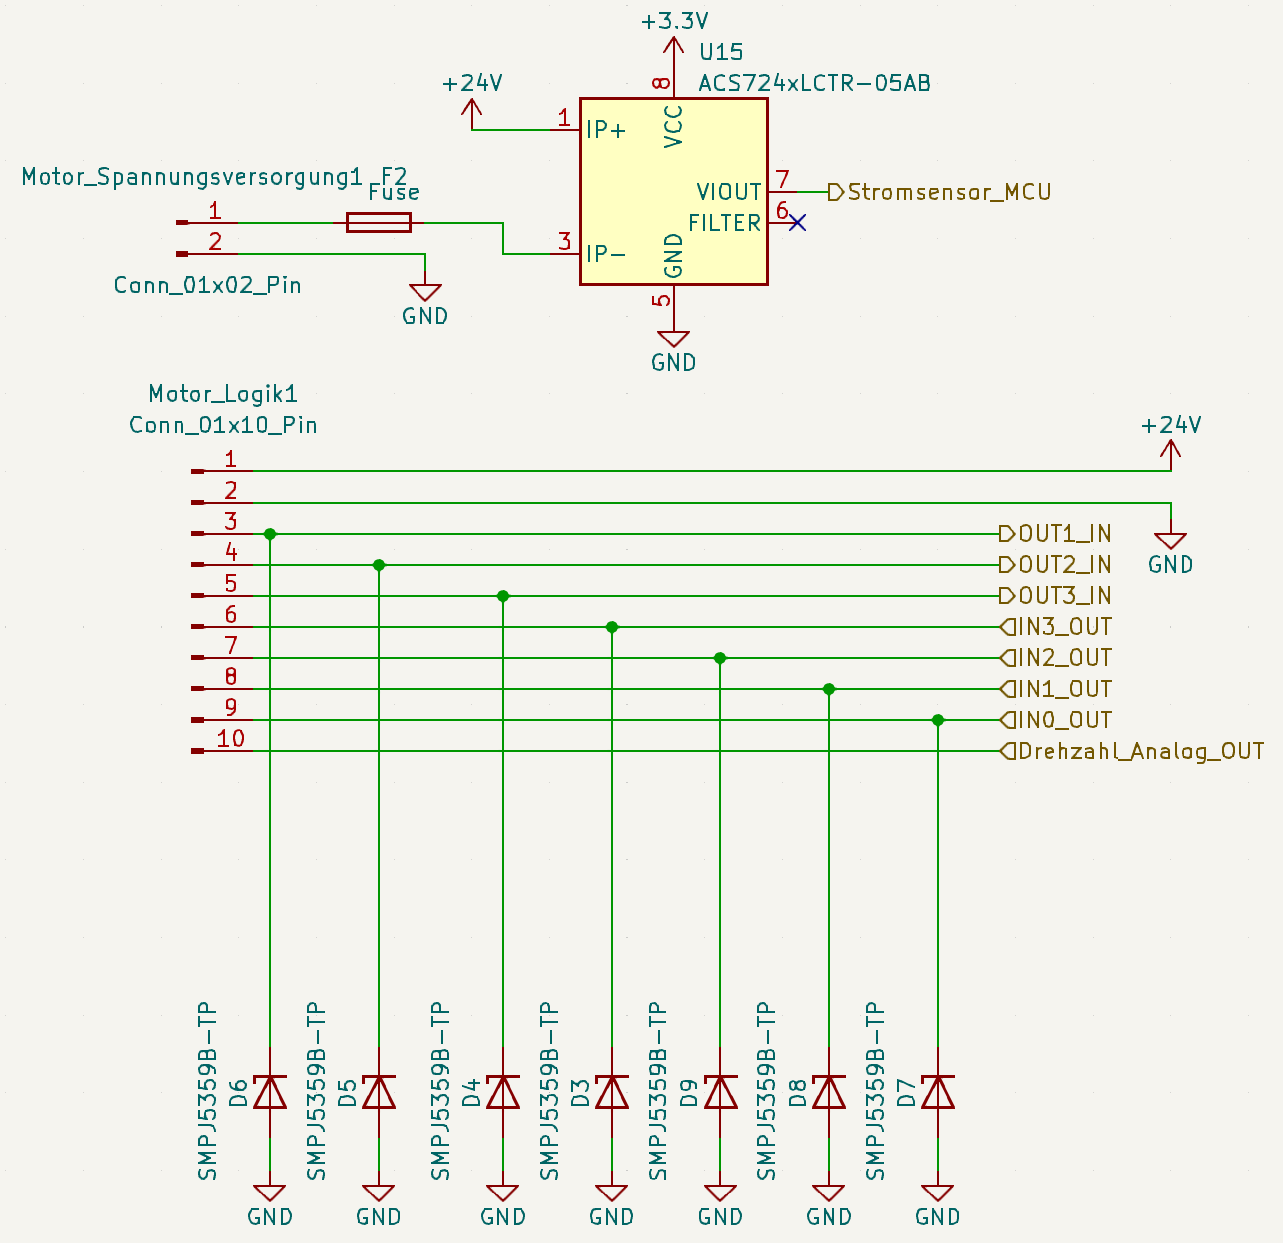
\includegraphics[width=1.0\textwidth]{images/Hardware/Motor_Schaltplan.PNG}
	\caption{Schaltplan der Motor Gruppe}
	\label{fig:MotorGruppe}\begin{center}
	\end{center}
\end{figure}
\subsection{Schaltplan Endschalter Gruppe}
\begin{figure}[H]
	\centering
	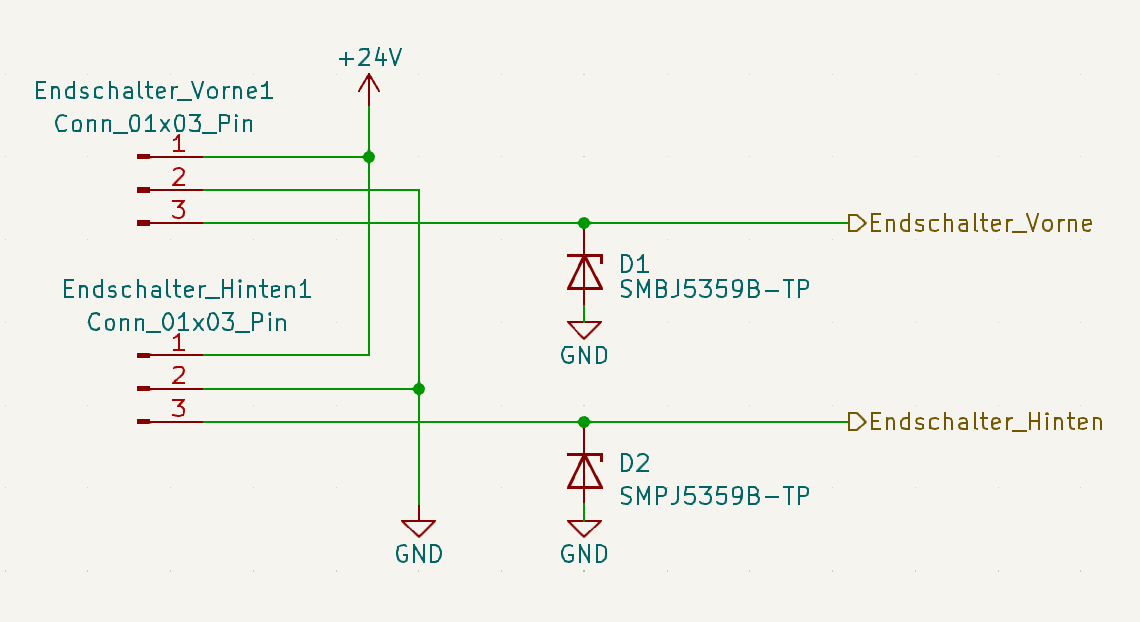
\includegraphics[width=1.0\textwidth]{images/Hardware/Endschalter_Schaltplan.PNG}
	\caption{Schaltplan der Endschalter Gruppe}
	\label{fig:EndschalterGruppe}\begin{center}
	\end{center}
\end{figure}´
\section{Bauteilliste}
\label{sec:Bauteilliste}
% Please add the following required packages to your document preamble:
% \usepackage{graphicx}
\begin{table}[H]
	\centering
	\resizebox{\textwidth}{!}{%
		\begin{tabular}{|l|l|l|}
			\hline
			\textbf{Bauteilbezeichnung} & \textbf{Bauteilart} & \textbf{Anzahl} \\ \hline
			Schurter TASTER 1104 GN & Button, Grün & 1 \\ \hline
			Schurter TASTER 1104 SW & Button, Schwarz & 2 \\ \hline
			LM3940IMP-3.3/NOPBCT-ND & Festspannungsregler & 1 \\ \hline
			FM25L16B-GTRCT-ND & F-RAM & 1 \\ \hline
			C1Q 4 & Fuse 1206, 4A & 1 \\ \hline
			3413.0223.22 & Fuse 1206, 5A & 1 \\ \hline
			RP1465 & Gehäuse & 1 \\ \hline
			R-78E5.0-0.5 & DC/DC Wandler & 1 \\ \hline
			Phoenix Contact 1984617 & Schraubterminal 2 Fach 3.5mm & 2 \\ \hline
			OSTVN02A150 & Schraubterminal 2 Fach 2.54mm & 3 \\ \hline
			OSTVN03A150 & Schraubterminal 3 Fach 2.54mm & 4 \\ \hline
			TE Connectivity 282834-7 & Schraubterminal 7 Fach  2.54mm & 1 \\ \hline
			OSTVN10A150 & Schraubterminal 10 Fach 2.54mm & 1 \\ \hline
			LM2904QS-13DICT-ND & Operationsverstärker & 1 \\ \hline
			MAX3485CSA+CT-ND & RS-485 Converter & 1 \\ \hline
			TMCS1101A3BQDRQ1CT-ND & Stromsensor & 1 \\ \hline
			LTST-C150GKT & SMD LED Grün & 3 \\ \hline
			LTST-C150KSKT & SMD LED Gelb & 3 \\ \hline
			LTST-C230KRKT & SMD LED Rot & 1 \\ \hline
			LTST-C230KFKT & SMD LED Orange & 1 \\ \hline
			LTV-817S & Optokoppler & 9 \\ \hline
			G6S-2F 24DC & Relais, 24V & 2 \\ \hline
			KDZVTR24BCT-ND & Zenerdiode, 24V & 9 \\ \hline
			Schurter FRONTSATZ & Button, Montagesatz & 3 \\ \hline
			C6000ALBB & Schalter & 1 \\ \hline
			C6000ALBB-1229W & Schalter, gekennzeichnet & 1 \\ \hline
			SL 2X10G SMD2,54 & Pin-Header, SMD & 1 \\ \hline
			SL 2X50G 2,54 & Pin-Header & 1 \\ \hline
			MEN 1216.1001 & LED-Lichtleiter & 8 \\ \hline
			KDZVTR6.8B & Zenerdiode, 6.8V & 4 \\ \hline
			IPG-2227 & Kabelverschraubung 3mm-6mm & 4 \\ \hline
			IPG-222135 & Kabelverschraubung 6mm-12mm & 4 \\ \hline
		\end{tabular}%
	}
	\caption{Bauteilliste Teil 1}
	\label{tab:Verwendeten Bauteile}
\end{table}

\begin{table}[H]
	\centering
	\begin{tabular}{|l|l|}
		\hline
		\textbf{Widerstände SMD1206} & \textbf{Anzahl} \\ \hline
		150$\Omega$ & 7 \\ \hline
		10k$\Omega$ & 5 \\ \hline
		120$\Omega$ & 4 \\ \hline
		750$\Omega$ & 2 \\ \hline
		240$\Omega$ & 1 \\ \hline
		700$\Omega$ & 6 \\ \hline
		11k$\Omega$ & 6 \\ \hline
		2,2k$\Omega$ & 3 \\ \hline
		6,8k$\Omega$ & 3 \\ \hline
		36k$\Omega$ & 3 \\ \hline
		110$\Omega$ & 1 \\ \hline
		2,3k$\Omega$ & 1 \\ \hline
		1k$\Omega$ & 1 \\ \hline
		\textbf{Kondensatoren SMD1206} &  \\ \hline
		22$\mu$F & 1 \\ \hline
		22nF & 6 \\ \hline
		220nF & 3 \\ \hline
		33$\mu$F & 1 \\ \hline
		0.47$\mu$F & 1 \\ \hline
	\end{tabular}
	\caption{Bauteilliste Teil 2}
	\label{tab:Bauteile2}
\end{table}
\newpage
\section{Valide URL und JSON Formate}
\label{sec:REST}
\subsection{GET-Anfragen}
\subsubsection{GET /data}
\begin{lstlisting}[language=XML, caption={GET-Request 1}]
{
	"error": <(int) error_code>,
	"operating_mode": <(int) 0/1 [manual/automatic]>,
	"localized": <(boolean)>,
	"sail_pos": <(int) pitch/roll [+/- 0...100 %]>,
	"wind": {
		"speed": <(int) speed[m/s]>,
		"direction": <(int) direction[degree]>
	},
	"current": <(int) current[mA]>
}
\end{lstlisting}
\subsubsection{GET /data/status}
\begin{lstlisting}[language=XML, caption={GET-Request 2}]
	{
		"error": <(int) error_code>,
		"operating_mode": <(int) 0/1 [manual/automatic]>,
		"localized": <(boolean)>,
	}
\end{lstlisting}
\subsubsection{GET /data/adjustment}
\begin{lstlisting}[language=XML, caption={GET-Request 3}]
	{
		"sail_pos": <(int) pitch/roll [+/- 0...100 %]>
	}
\end{lstlisting}
\newpage
\subsubsection{GET /data/sensors}
\begin{lstlisting}[language=XML, caption={GET-Request 4}]
	{
		"wind": {
			"speed": <(int) speed[m/s]>,
			"direction": <(int) direction[degree]>
		},
		"current": <(int) current[mA]>
	}
\end{lstlisting}
\subsubsection{GET /data/settings}
\begin{lstlisting}[language=XML, caption={GET-Request 5}]
	{
		"max_rpm": <(int) 400 - 2000>,
		"max_distance_error": <(int) 5 - 50>
	}
\end{lstlisting}

\subsection{PUT-Anfragen}
\subsubsection{PUT /data/status/error}
\begin{lstlisting}[language=XML, caption={PUT-Request 1}]
	{
		"error": <(int) error_code>,
	}
\end{lstlisting}
\newpage
\subsubsection{PUT /data/adjustment}
\begin{lstlisting}[language=XML, caption={PUT-Request 2}]
	{
		"sail_pos": <(int) pitch/roll [+/- 0...100 %]>
	}
\end{lstlisting}
\subsubsection{PUT /data/status/operating\_mode}
\begin{lstlisting}[language=XML, caption={PUT-Request 3}]
	{
		"operating_mode": <(int) 0/1 [manual/automatic]>
	}
\end{lstlisting}
\subsubsection{PUT /data/settings}
\begin{lstlisting}[language=XML, caption={PUT-Request 4}]
	{
		"max_rpm": <(int) 400 - 2000>,
		"max_distance_error": <(int) 5 - 50>
	}
\end{lstlisting}